%\documentclass[12pt,a4paper]{report}
\documentclass[12pt,a4paper,oneside,onecolumn,openright]{book}
% set the document language
\usepackage[italian]{babel}
% set the encoding used by your editor here (default is utf8)
\usepackage[utf8]{inputenc}
\usepackage[T1]{fontenc}

% math packages
\usepackage{amsmath}
\usepackage{amssymb}
% page margins settings
\usepackage[inner=3cm,outer=2.5cm,top=3cm,bottom=2.5cm]{geometry}
%\usepackage{indentfirst}

% other packages
\usepackage[table]{xcolor}
\usepackage{float}
\usepackage{array}
\usepackage{subfigure}
\usepackage{graphicx}
\usepackage{verbatim}
\usepackage{listings}
\usepackage{url}
\usepackage{pythontex}
\usepackage[hidelinks]{hyperref}
% custom colors
\usepackage{color}
\definecolor{light-gray}{gray}{0.96}
\definecolor{cyan}{RGB}{230,230,255}
\definecolor{dkgreen}{rgb}{0,0.6,0}
\definecolor{gray}{rgb}{0.5,0.5,0.5}
\definecolor{mauve}{rgb}{0.58,0,0.82}

% environment for bash code
\lstset{ %
  language=bash,                % the language of the code
  basicstyle=\footnotesize,           % the size of the fonts that are used for the code
  numbers=left,                   % where to put the line-numbers
  numberstyle=\footnotesize,          % the size of the fonts that are used for the line-numbers
  stepnumber=1,                   % the step between two line-numbers. If it's 1, each line 
                                  % will be numbered
  numbersep=5pt,                  % how far the line-numbers are from the code
  backgroundcolor=\color{white},      % choose the background color. You must add \usepackage{color}
  showspaces=false,               % show spaces adding particular underscores
  showstringspaces=false,         % underline spaces within strings
  showtabs=false,                 % show tabs within strings adding particular underscores
%  frame=single,                   % adds a frame around the code
  rulecolor=\color{black},        % if not set, the frame-color may be changed on line-breaks within not-black text (e.g. commens (green here))
  tabsize=2,                      % sets default tabsize to 2 spaces
  captionpos=b,                   % sets the caption-position to bottom
  breaklines=true,                % sets automatic line breaking
  breakatwhitespace=false,        % sets if automatic breaks should only happen at whitespace
  title=\lstname,                   % show the filename of files included with \lstinputlisting;
                                  % also try caption instead of title
  numberstyle=\tiny\color{gray},        % line number style
  keywordstyle=\textbf,          % keyword style
  commentstyle=\color{dkgreen},       % comment style
%  stringstyle=\color{mauve},         % string literal style
  escapeinside={\%*}{*)},            % if you want to add a comment within your code
  morekeywords={*,...,insert,-}               % if you want to add more keywords to the setù
}

% environment for python code
\lstset{
language=Python,
breaklines=true,
breakatwhitespace=true ,
backgroundcolor=\color{light-gray}
}
% appendices package
%\usepackage{appendix}
% set Appendix name used in the toc
%\renewcommand{\appendixtocname}{Appendice}

% interline
\linespread{1.5}
% set numbers for subsections and show them in the toc
\setcounter{tocdepth}{3} 
\setcounter{secnumdepth}{3}

% layout package, style and settings
\usepackage{fancyhdr}
\pagestyle{fancy}

\fancypagestyle{mainmatter}{%		
		\fancyhf{} 
		\fancyhead{}
		\fancyhead[LE,RO]{\thepage}
		\fancyhead[LO]{\footnotesize{\leftmark}}
		\fancyhead[RE]{\footnotesize{\rightmark}}
		\fancyfoot{}
		\addtolength{\headwidth}{\marginparsep}
		\addtolength{\headheight}{2.5pt}
		\renewcommand{\headrulewidth}{0.3pt}
		\renewcommand{\footrulewidth}{0.0pt}
		}
\fancypagestyle{frontmatter}{%
		\fancyhf{} 
		\fancyhead[LE]{\footnotesize{\MakeUppercase{\thepage}}}
		\fancyhead[RO]{\footnotesize{\MakeUppercase{\thepage}}}
		\fancyhead[RE,LO]{}
		\fancyfoot{}
		\addtolength{\headwidth}{\marginparsep}
		\addtolength{\headheight}{2.5pt}
		\renewcommand{\headrulewidth}{0.0pt}
		\renewcommand{\footrulewidth}{0.0pt}
		}
		
		
\usepackage{fancyhdr}
\pagestyle{fancy}
		\fancyhf{} 
		\fancyhead{}
		\fancyhead[LE,RO]{\thepage} 
		\fancyhead[LO]{\footnotesize{\leftmark}}
		\fancyhead[RE]{\footnotesize{\rightmark}}
		\fancyfoot{}
		\addtolength{\headwidth}{\marginparsep}
		\addtolength{\headheight}{2.5pt}
		\renewcommand{\headrulewidth}{0.3pt}
		\renewcommand{\footrulewidth}{0.0pt}

	\graphicspath{ {images/} }
% empty pages have no numbers
\makeatletter
\def\cleardoublepage{\clearpage\if@twoside \ifodd\c@page\else
\hbox{}
  %Potresti voler togliere il commento dalla linea seguente
  %Questa pagina � stata lasciata intenzionalmente vuota.
\thispagestyle{empty}
\newpage
\if@twocolumn\hbox{}\newpage\fi\fi\fi}
\makeatother
%????
%\textwidth=450pt\oddsidemargin=0pt

%\makeatletter 
%  \DeclareRobustCommand*\textsubscript[1]{% 
%    \@textsubscript{\selectfont#1}} 
%  \newcommand{\@textsubscript}[1]{% 
%    {\m@th\ensuremath{_{\mbox{\fontsize\sf@size\z@#1}}}}} 
\makeatother 

\begin{document}

\begin{titlepage}
\begin{center}
{
    \large
    \textbf{Università  degli studi di Modena e Reggio Emilia} \\
   	\textbf{Dipartimento di Scienze Fisiche, Informatiche e Matematiche} \\
    \vspace{\stretch{0.5}}
    \hspace*{0cm} \hrulefill \hspace*{0cm} \\
    \vspace{\stretch{0.5}}
   	\emph{Corso di Laurea in Informatica}
    
	  \vspace{\stretch{12}}
  
  
 		\huge{\bf Fingerprinting tramite analisi  
 			 }}\\
		\vspace{3mm}
		\vspace{3mm}
		{\huge{\bf di protocolli di rete}}\\
		\vspace{3mm}
		\vspace{3mm}
		{\huge{\bf e strategie di offuscamento}}\\
		\vspace{3mm}
		\vspace{3mm}
		
		\vspace{\stretch{6}}
		\end{center}
		
\vspace{40mm}
\par
\noindent
\begin{minipage}[t]{0.47\textwidth}
{\large{\bf Relatore:\\
Luca Ferretti}}\\ 
\\

\end{minipage}
\hfill
\begin{minipage}[t]{0.47\textwidth}\raggedleft
{\large{\bf Candidato:\\
Fabio Zanichelli}}
\end{minipage}
\vspace{20mm}
\begin{center}
%\rule[0.1cm]{15.8cm}{0.1mm}
\hspace*{0cm} \hrulefill \hspace*{0cm} \\
{\large{\bf 
Anno Accademico 2021/2022}}
\end{center}

\end{titlepage}

\pagestyle{frontmatter}
\frontmatter

 %PAGINA VUOTA
\clearpage\null\thispagestyle{empty}\clearpage
\setcounter{tocdepth}{2}
\tableofcontents

\setlength{\parindent}{12pt}
\setlength{\parskip}{1ex plus 0.5ex minus 0.2ex}
\mainmatter
\pagestyle{mainmatter}



\chapter{Introduzione}
\label{introduzione}

\section{OS Fingerprinting}
\label{citazioni}

L'OS fingerprinting consiste nel rilevare da remoto il sistema operativo di un dispositivo analizzandone i pacchetti inviati. Le differenze di implementazione dello stack TCP/IP, infatti, determinano comportamenti diversi che, analizzati, consentono di ottenere informazioni utili a questo scopo. \\
Il fingerprinting può essere effettuato in due modalità: attiva e passiva. \\ 
Nella prima si analizzano le risposte ricevute in seguito ad alcuni pacchetti inviati; questi sono appositamente costruiti in modo da massimizzare le informazioni che si possono ottenere dalla risposta.
Nella seconda, invece, viene ispezionato il normale traffico del dispositivo target; si tratta quindi di una tecnica meno invasiva e che si espone meno al rischio di essere scoperti.

\section{Obiettivo}
L'obiettivo consiste nell'analizzare le differenze che portano all'individuazione del sistema operativo, e successivamente modificare determinati parametri di quest'ultimo in modo da riuscire ad ingannare i principali strumenti per il fingereprinting.
I risultati ottenuti, quindi, dovranno essere errati e portare all'individuazione di un sistema operativo differente rispetto a quello realmente in uso.\\
Si è proceduto utilizzando un server HTTP, gestendo quindi pacchetti di non cifrati; si è successivamente cercato di effettuare un'analisi sull'handshake TLS, ovvero sullo scambio di messaggi che precede una comunicazione cifrata.

\section{Strumenti e sistemi operativi utilizzati}
Per la realizzazione dell'obiettivo sono stati utilizzati due differenti sistemi operativi: Windows 11 e Kali (una distribuzione Linux basata su Debian).
La motivazione della scelta di questi sistemi risiede nel fatto che Kali sia stato progettato per la sicurezza informatica, e Windows sia il sistema operativo attualmente più utilizzato; per questa ragione, l'individuazione di quest'ultimo (seppur falsificata) desterebbe meno sospetti. 

I tool utilizzati sono stati i seguenti:
\begin{itemize}
	\item \textbf{Nmap}: principale strumento per effettuare fingerprinting attivo tramite l'invio di specifici pacchetti (\textit{probe}) costruiti appositamente per massimizzare le differenze tra i comportamenti dei sistemi operativi. Consente inoltre di effettuare altre operazioni, alcune delle quali fondamentali per il fingerprinting stesso, come ad esempio il port scanning.
	\item \textbf{p0f}: tool per effettuare fingerprinting passivo. Esso analizza solamente i pacchetti ricevuti da una determinata interfaccia o analizza quelli passati tramite un file con estensione pcap. È anche in grado di effettuare fingerprinting a livello 7.
	\item \textbf{Wireshark}: si tratta di uno strumento che permette la visualizzazione dei pacchetti inviati e ricevuti dal dispositivo tramite un'interfaccia grafica. Consente inoltre di filtrare pacchetti sulla base di determinati campi o protocolli utilizzati.
	\item \textbf{Server Apache}: Web server che consente di rispondere alle richieste di tipo HTTP/HTTPS. È stato installato sia su Windows 11 che su Kali per poter effettuare il confronto tra le risposte inviate.
	\item \textbf{Scapy}: libreria Python in grado di inviare pacchetti modificabili in ogni campo. Molto utile il suo utilizzo per quanto riguarda l'invio di pacchetti "patologici" che stimolano risposte utili ai fini del fingerprinting.
	\item \textbf{nftables}: tool per che permette la modifica o il blocco di pacchetti sulla base del loro contenuto negli header.
\end{itemize}

	







\chapter{Base knowledge}

Per effettuare comunicazioni tramite internet, vi è il bisogno che tutti i dispositivi connessi rispettino determinati meccanismi; questo si rende necessario a causa dell'elevata eterogeneità derivata da hardware e software differenti.
Questi meccanismi, che prendono il nome di \textit{protocolli}, sono strutturati secondo diversi layer (livelli) formando lo stack TCP/IP.  \\
Sebbene l'idea originale (modello ISO/OSI) prevedesse un modello composto da sette livelli, de facto lo schema attualmente in uso ne prevede solamente quattro. Nonostante ciò, nella terminologia informatica la numerazione dei livelli è rimasta quella precedente.
\\
\begin{table}[htb]
	\centering
	\begin{tabular}{| l | c |}
		\hline
		Livello 7 & Applicativo
		\\
		\hline
		Livello 4 & Trasporto
		\\
		\hline
		Livello 3 & Rete
		\\
		\hline
		Livello 2 & Fisico
		\\
		\hline
		
	\end{tabular}
	\caption{Livelli dello stack TCP/IP}
	\label{tab:stack}
\end{table}

\section{Funzionamento dello stack TCP/IP}
Il meccanismo dello stack prevede che ad ogni livello vengano aggiunte al messaggio delle intestazioni (header), a partire dal layer più alto, che verranno valutate dal medesimo livello del ricevente.
Si precisa che l'ordine in cui si valutano gli header dei livelli è inverso rispetto a quello del mittente; il ricevente partirà infatti dal livello più basso.
Questa procedura prende il nome di \textit{incapsulamento} ed è riassunta nella seguente figura:


\begin{figure}[h]
	\centering
	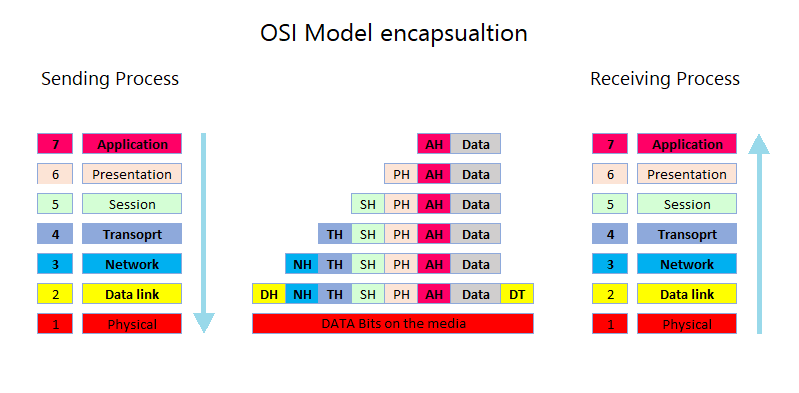
\includegraphics[width=\textwidth]{figures/incapsulamento.png}
	\caption{Incapsulamento nel modello ISO/OSI}
	\label{incapsulamento}
	\cite{incapsulamento}
\end{figure}

\section{Header per il fingerprinting}
Gli header aggiunti ad ogni livello sono formati da vari campi contententi informazioni utili per la comunicazione, e il valore che questi assumono in determinate situazioni è dipendente dal sistema operativo che si sta utilizzando.

Si prenda ad esempio l'header TCP, un protocollo del livello 4 dello stack:\\

\begin{figure}[H]
	\centering
	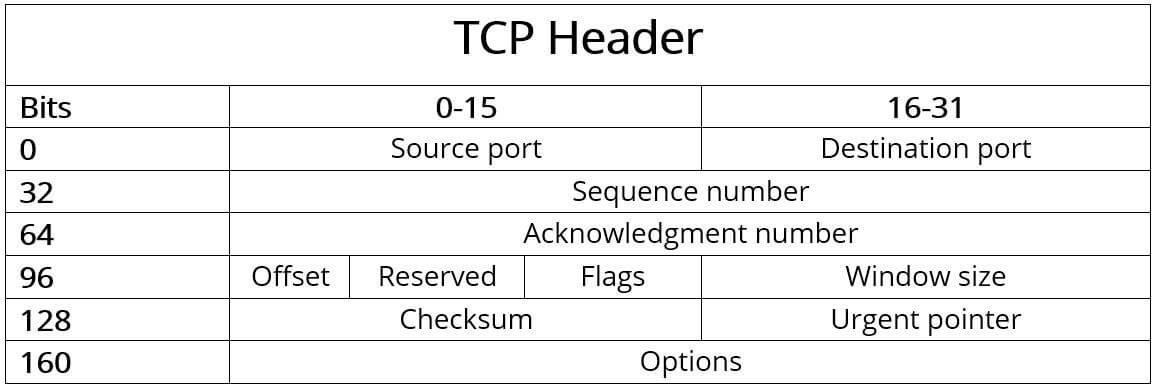
\includegraphics[width=\textwidth]{figures/headerTCP.JPG}
	\caption{Header TCP}
	\label{headerTCP}
	\cite{headerTCP}
\end{figure}

Il campo \textit{option} permette di segnalare al ricevente l'uso di alcune opzioni di comunicazione; il loro supporto e l'effettivo utilizzo, essendo queste facoltative e quindi peculiari di specifici sistemi operativi, rivestono quindi particolare importanza ai fini del fingerprinting.
Esempi analoghi si possono trovare nei protocolli ad ogni livello dello stack, e l'unione delle informazioni acquisite dall'analisi degli header consente di poter individuare con una discreta precisione il sistema operativo del dispositivo target.
\chapter{Analisi}

\section{Procedura}
%L'attività di analisi iniziale, ovvero senza l'ausilio di librerie specifiche per l'invio di determinati pacchetti, è stata effettuata installando un server Apache sia su Windows 11 che su Kali.
%Si è quindi proceduto ad inviare richieste ai server tramite browser web e all'analisi dei pacchetti ricevuti in risposta con l'utilizzo di Wireshark.
%Successivamente sono state analizzate anche le risposte a determinati pacchetti inviati utilizzando la libreria Scapy.
%Di seguito sono riportate le differenze più importanti rilevate durante l'intera attività di analisi.
L'analisi dei pacchetti per l'individuazione delle differenze è stata effettuata sulle risposte ricevute da server Apache installati su Windows 11 e su Kali.
L'attività si analisi è stata svolta in due differenti modalità:
\begin{enumerate}
	\item Nella prima sono state analizzate le risposte ricevute in seguito a richieste GET HTTP inviate tramite browser web; la cattura e l'osservazione di queste è stata effettuata tramite Wireshark.
	\item Nella seconda si è proceduto con l'ispezione delle risposte a specifici pacchetti inviati utilizzando la funzione \textit{sr1} della libreria Python Scapy, che permette la cattura della risposta al pacchetto inviato. Le risposte sono state esaminate con la funzione \textit{show}.
\end{enumerate}
Di seguito vengono mostrate le principali differenze notate tra i due sistemi operativi durante l'intera attività di analisi.

\section{Livello 3: protocolli IP e ICMP}
È stata effettuata in primis l'analisi del TTL (\textit{Time To Live}), essendo un valore estremamente semplice da analizzare.
Questo campo contiene un numero intero positivo che viene decrementato ad ogni \textit{hop}, ovvero ad ogni router che il pacchetto incontra nel percorso verso l'host ricevente, e viene eliminato dalla rete quando questo raggiunge lo 0.
Il protocollo, però, non impone nessun valore di partenza, lasciando libertà di scelta al sistema operativo del mittente; l'unico limite è rappresentato dagli 8 bit riservati a quel campo (ovvero ad un valore massimo di 255).
L'analisi ha portato ad evidenziare la seguente differenza riguardo al TTL:
\begin{table}[H]
	\centering
	\begin{tabular}{| l | c |}
		\hline
		\rowcolor{blue!10} Windows 11 & 128
		\\
		\hline
		\rowcolor{red!10} Kali & 64
		\\
		\hline
		
	\end{tabular}
	\caption{TTL iniziale}
	\label{tab:TTL}
\end{table}

Questa differenza è molto importante in quanto è presente in ogni pacchetto inviato in rete e, se non vengono apportate modifiche, non varia tra un pacchetto e l'altro. Solitamente i valori iniziali sono potenze di due (64 o 128); l'eventuale utilizzo di valori parecchio inusuali denota un comportamento molto riconoscibile.
\\
\\
Inoltre, è stata effettuata l'analisi del protocollo ICMP, e in particolare è stata notata una differenza nel campo \textit{code} in caso di risposta a determinati pacchetti inviati utilizzando la libreria di Python scapy.

\begin{lstlisting}[language=Python, caption={Comando Python per l'invio del pacchetto}]
	from scapy.all import *
	
	pkt = sr1(IP(dst='192.168.63.1')/ICMP(code=9))
	pkt.show()
	
\end{lstlisting}
Questo comando invia un pacchetto ICMP con il campo \textit{code} impostato ad un numero casuale, in questo caso 14: in questo specifico contesto, Windows 11 risponde inviando un pacchetto in cui \textit{code}=0, mentre Kali copia il valore che ha ricevuto nella richiesta.

\begin{table}[h]
	\centering
	\begin{tabular}{ | l | c |}
		\hline
		\rowcolor{blue!10} Windows 11 & 0
		\\
		\hline
		\rowcolor{red!10} Kali & Stesso valore inviato nella richiesta
		\\
		\hline

	\end{tabular}
	\caption{Campo code quando nella richiesta è diverso da 0}
	\label{tab:code}
\end{table}

La differenza è molto peculiare perchè riconoscibile utilizzando solamente il protocollo ICMP (lo stesso del comando \textit{ping}) e non ne influenza il normale utilizzo dal momento che la differenza si presenta solo inviando determinati pacchetti \textit{echo request}.
\section{Livello 4: analisi protocollo TCP}
Il livello 4 dello stack è formato da due protocolli: User Datagram Protocol (UDP) e Transmission Control Protocol (TCP). Entrambi forniscono informazioni utili per il fingerprinting, ma il TCP possiede un numero maggiore di campi e di opzioni utilizzabili, pertanto è stata data priorità all'analisi di quest'ultimo.

Analizzando l'handshake TCP, si può notare una discrepanza nell'utilizzo del Window Scale; quest'opzione consente di aumentare la Window Size oltre il valore che si otterrebbe settando tutti i bit di quel campo a 1.
Ciò è dovuto al fatto che il valore dell'opzione rappresenta il numero di shift verso sinistra dei bit del Window Size, che corrispondono a raddoppi del valore contenuto. 
L'utilizzo di questa opzione viene concordato nei segmenti SYN e SYN+ACK dell'handshake e il suo valore non viene più modificato per il resto della connessione. Confrontando i valori ottenuti da Windows 11 e Kali, si ottiene il seguente risultato:
\\
\begin{table}[htb]
	\centering
	\begin{tabular}{| l | c |}
		\hline
		\rowcolor{blue!10} Windows 11 & 8
		\\
		\hline
		\rowcolor{red!10} Kali & 7
		\\
		\hline
		
	\end{tabular}
	\caption{Window Scaling Factor}
	\label{tab:Window Scale}
\end{table}

Si tratta di una differenza importante, la quale però per essere rilevata necessita del livello 4 dello stack; inoltre, si può osservare solo se si utilizza il protocollo TCP, essendo UDP privo di handshake.
\\
\\
Proseguendo l'analisi si possono notare ulteriori differenze riguardanti il flag sulla notifica esplicita di congestione (ECN). Si tratta di un flag che consente di comunicare a livello end to end una congestione, evitando però la perdita dei pacchetti. Il mittente, infatti, se riceve un pacchetto contenente quest'informazione diminuisce i pacchetti inviati in quella comunicazione, seguendo specifici algoritmi (ad esempio, Reno). 
Se si invia un pacchetto simulando l'inizio di un handshake (SYN) con i flag sulla congestione attivi e si osserva la risposta (SYN+ACK), si possono notare risultati differenti tra i pacchetti ricevuti da Windows 11 e Kali:
\\
\begin{lstlisting}[language=Python, caption={Comando Python per l'invio del pacchetto}]
	from scapy.all import *
	
	pkt=sr1(IP(dst='192.168.63.1')/TCP(dport=80, flags='SCE'))
	pkt.show()
	
\end{lstlisting}

\begin{table}[h]
	\centering
	\begin{tabular}{| l | c |}
		\hline
		\rowcolor{blue!10} Windows 11 & 0
		\\
		\hline
		\rowcolor{red!10} Kali & 1
		\\
		\hline
		
	\end{tabular}
	\caption{ECN in risposta a specifico pacchetto}
	\label{tab:ECN}
\end{table}

Questa diversità è molto importante per il fingerprinting di Nmap che, come verrà meglio specificato nella sezione \ref{algoritmi}, assegna una punteggio elevato al risultato di questo test. 

\section{Livello 7: analisi protocollo HTTP}
Sebbene HTTP sia un protocollo a livello applicativo, esso consente ugualmente di ricavare alcune informazioni utili per l'OS fingerprinting: il campo \textit{User-Agent}, infatti, contiene informazioni esplicite riguardanti il browser che si sta utilizzando e il sistema operativo in utilizzo. Questo tipo di situazione prende il nome di \textit{banner grabbing}.

Inoltre, a questo livello dello stack si può tentare un fingerprinting che vada oltre l'individuazione del sistema operativo, ponendo come obiettivo quello di indovinare il tipo di applicativo in uso.
Questo è reso possibile dal fatto che HTTP è un protocollo di tipo testuale, pertanto non vi sono campi prefissati in determinati bit per ogni funzione.
L'header, infatti, contiene varie coppie secondo lo schema:\\
\textbf{chiave:valore} 


Questo, a differenza dei protocolli analizzati precedentemente, permette un diverso ordine con le quali le coppie vengono elencate, essendo questo ininfluente per una corretta comunicazione; ne consegue che analizzare l'ordinamento è molto importante se si vuole tentare di individuare, ad esempio, il tipo di client in utilizzo.\\

Osservando i pacchetti HTTP inviati dai principali browser web si possono notare delle differenze sull'ordinamento per quanto riguarda Firefox e altri browser basati su Chromium.
L'ordine dei campi nell'header è infatti il seguente:

\begin{table}[h]
	\centering
	\begin{tabular}{| c | c |}
		\hline
		\textbf{Firefox} & \textbf{Chromium-based}
		\\
		\hline
		Host & Host
		\\
		\hline
		User-Agent & Connection
		\\
		\hline
		Accept & Upgrade-Insecure-Requests
		\\
		\hline
		Accept-language & User-Agent
		\\
		\hline
		Accept-Encoding & Accept
		\\
		\hline
		Connection & Accept-Encoding
		\\
		\hline
		Upgrade-Insecure-Requests & Accept-Language
		\\
		\hline
	\end{tabular}
	\caption{Ordine campi header HTTP}
	\label{tab:ordineHTTP}
\end{table}

Inoltre, analizzando i linguaggi accettati si possono osservare ulteriori disuguaglianze riguardanti il campo \textit{Quality Value}.
Si tratta di un valore indicato tramite la lettera q (case insensitive) che esprime la preferenza a determinati linguaggi tramite un numero compreso tra 0 e 1, avente massimo tre cifre decimali; il valore di default è 1 ovvero la massima preferenza \cite{qvalue}. 

Segue la stringa di quello specifico campo riguardante Chrome e Firefox:

\begin{lstlisting} [caption={Campo Accept-Language di Chrome}]
	Acceept-Language: it-IT,it;q=0.9,en-US;q=0.8,en;q=0.7
\end{lstlisting}

\begin{lstlisting}[caption={Campo Accept-Language di Firefox}]
	Acceept-Language: it-IT,it;q=0.8,en-US;q=0.5,en;q=0.3
\end{lstlisting}

Si possono dunque distinguere delle differenze tra i due browser, che ovviamente possono rivestire un ruolo importante in fase di fingerprinting dello User-Agent utilizzato.
\\

È possibile, inoltre, osservare ulteriori differenze che vi sono tra i due browser analizzando il campo \textit{Accept} dell'Header HTTP. Si osservino infatti i due campi nei due browser web menzionati precedentemente:
\\


\begin{lstlisting}[caption={Campo \textit{Accept} di richiesta GET di Chrome}]
	text/html,application/xhtml+xml,application/xml;q=0.9,image/avif,
	image/webp,image/apng,*/*;q=0.8,application/signed-exchange;v=b3;q=0.9
\end{lstlisting}

\begin{lstlisting}[caption={Campo \textit{Accept} di richiesta GET di Firefox}]
	text/html,application/xhtml+xml,application/xml;q=0.9,image/avif,
	image/webp,*/*;q=0.8
\end{lstlisting}

















\chapter{Offuscamento}

In questa capitolo si ha l'obiettivo di ingannare i tool di figerprinting, portandoli ad un risultato errato. Più precisamente, si ha lo scopo di modificare parametri di Kali per ottenere il riconoscimento di Windows.
\\
Non essendo Windows 11 presente nel database di Nmap e non potendo quindi essere un risultato del fingerprinting, si cercherà di portare i tool all'individuazione della sua versione precedente, ovvero Windows 10.

\section{Algoritmo utilizzato da Nmap} \label{algoritmi}
Prima di procedere occorre precisare il funzionamento dell'algoritmo di Nmap per il riconoscimento dei sistemi operativi. Questo avviene secondo un meccanismo di punteggi che viene dato ad ogni test effettuato, specificato nella prima entry del database. I test che non ottengono alcun risultato utile non vengono conteggiati nel totale dei punti.
A questo punto, vi sono due possibili situazioni:
\begin{itemize}
	\item Se i risultati dei test combaciano perfettamente con quelli di una entry del database, allora quella verrà mostrata come risultato finale,
	\item Se i risultati dei test non coincidono con nessun sistema operativo, allora verranno calcolati i punti di ogni test soddisfatti per ogni sistema; quello con cui è stato realizzato un numero maggiore di punti sarà quello mostrato.
\end{itemize}

Segue l'elenco di test con il relativo punteggio \footnote{Nmap OS Fingerprinting 2nd Generation DB, \url{https://svn.nmap.org/nmap/nmap-os-db}}:

\begin{lstlisting}[caption={Punteggi che Nmap attrribuisce ad ogni test}]
	MatchPoints
	SEQ(SP=25%GCD=75%ISR=25%TI=100%CI=50%II=100%SS=80%TS=100)
	OPS(O1=20%O2=20%O3=20%O4=20%O5=20%O6=20)
	WIN(W1=15%W2=15%W3=15%W4=15%W5=15%W6=15)
	ECN(R=100%DF=20%T=15%TG=15%W=15%O=15%CC=100%Q=20)
	T1(R=100%DF=20%T=15%TG=15%S=20%A=20%F=30%RD=20%Q=20)
	T2(R=80%DF=20%T=15%TG=15%W=25%S=20%A=20%F=30%O=10%RD=20%Q=20)
	T3(R=80%DF=20%T=15%TG=15%W=25%S=20%A=20%F=30%O=10%RD=20%Q=20)
	T4(R=100%DF=20%T=15%TG=15%W=25%S=20%A=20%F=30%O=10%RD=20%Q=20)
	T5(R=100%DF=20%T=15%TG=15%W=25%S=20%A=20%F=30%O=10%RD=20%Q=20)
	T6(R=100%DF=20%T=15%TG=15%W=25%S=20%A=20%F=30%O=10%RD=20%Q=20)
	T7(R=80%DF=20%T=15%TG=15%W=25%S=20%A=20%F=30%O=10%RD=20%Q=20)
	U1(R=50%DF=20%T=15%TG=15%IPL=100%UN=100%RIPL=100%RID=100%RIPCK=100%
	RUCK=100%RUD=100)
	IE(R=50%DFI=40%T=15%TG=15%CD=100)
\end{lstlisting}

Come si può notare, alcuni test hanno un valore maggiore rispetto ad altri per la frequenza con cui vengono svolti. Ad esempio il test T, che controlla il valore del TTL iniziale, viene effettuato nove volte mentre il test CD che verifica il campo code nel protocollo ICMP viene effettuato una sola volta.
Questa è una delle ragioni che spiega la discrepanza tra i punteggi attribuiti ai diversi test che vengono svolti.
Un ulteriore esempio di quanto appena affermato si può trovare tra i test della riga OPS (effettuati sulle opzioni TCP) e i test sulla riga U1, riguardanti il protocollo UDP.


\section{Modifiche al file sysctl.conf}
Per ottenere un sistema operativo differente, occorre modificare alcuni parametri del file sysctl.conf in modo da ottenere i valori di Windows.
La prima modifica riguarda il campo del TTL; variarlo da 64 a 128 consente di ingannare il test T, che calcola il valore iniziale di questo campo. La modifica vale per tutti i pacchetti che verranno inviati, quindi questo consente di spostare un grande quantità di punti a favore del riconoscimento di Windows, essendo il test ripetuto per molti pacchetti.

\begin{lstlisting}[caption={Modifica al campo TTL nel file sysctl.conf}, label=listing_ttl]
	net.ipv4.ip_default_ttl=128
\end{lstlisting}

Un'ulteriore modifica può essere effettuata per quanto riguarda il flag ECN, la cui differenza è stata spiegata nella sezione \ref{tab:ECN}. Questo riguarda i test della quarta riga, in cui quello specifico per la notifica esplicita di congestione ha un valore di 100 punti.

\begin{lstlisting}[caption={Modifica al campo ECN nel file sysctl.conf}]
	net.ipv4.tcp_ecn=0
\end{lstlisting} 

Il valore 0 significa che l'host non può accettare né inizializzare l'utilizzo del flag ECN. Il comportamento in risposta a determinati pacchetti "patologici" è ora simile a quello di Windows.

Si può inoltre procedere modificando il valore della Windows Size massima, causando di conseguenza un cambiamento del valore del Window Scaling Factor, da 7 a 8. 
La riga scritta nel file è la seguente:

\begin{lstlisting}[caption={Modifica alla Windows Size massima nel file sysctl.conf}, label=listingscaling]
	net.core.rmem_max = 8388608
\end{lstlisting}

Questa modifica, presa singolarmente, non influenza il risultato del fingerprinting in quanto questo campo è contenuto all'interno delle TCP options, che vengono valutate in maniera aggregata. Servono quindi ulteriori modifiche che verranno illustrate successivamente.

\section{Modifiche tramite nftables}
La modifica dei pacchetti in uscita dall'host di cui si vuole effettuare il fingerprinting tramite nftables consente il cambiamento del comportamento solo in determinate situazioni; di particolare interesse sono quelle riguardanti i probe di Nmap.
\\
La differenza mostrata alla tabella \ref{tab:code} è oggetto di uno dei test effettuati da Nmap. Quest'ultimo, infatti, invia un pacchetto \textit{echo request} con campo \textit{code} impostato a 9, e valuta la risposta ricevuta.
Questa dovrebbe essere zero nel caso di un \textit{echo reply}, ma questo comportamento è in realtà dipendente dal sistema operativo in utilizzo.
Manipolare i pacchetti echo reply in uscita per modificare il campo code nel caso questo sia 9 consente la variazione del risultato del test effettuato da Nmap. L'alto valore in termini di punteggio assegnato a questo test rende questa modifica molto importante ai fini dell'offuscamento.\\
Il comando per ottenere questo comportamento è contenuto nel file nftables.conf, nella tabella output.

\begin{lstlisting}[caption={Modifica del campo code in caso di test Nmap}, label=codice_icmp]
	icmp type 0 icmp code 9 icmp code set 0
\end{lstlisting}

Esaminando il database di Nmap, ci si accorge che vi è una differenza nel Window Size tra Kali e Windows 10. Modificare questo campo permette quindi di falsificare un altro test eseguito da Nmap, contribuendo quindi alla realizzazione dell'offuscamento.
Si procede dunque ad impostare la Window Size come descritta nel database.

\begin{lstlisting}[caption={Modifica della Window Size}, label=listingsize]
	tcp window != 0x2000 tcp window set 0x2000
\end{lstlisting}

Attuando tutte le modifiche elencate fino a questo punto, l'output di Nmap risulta essere il seguente:

\begin{figure}[H]
	\centering
	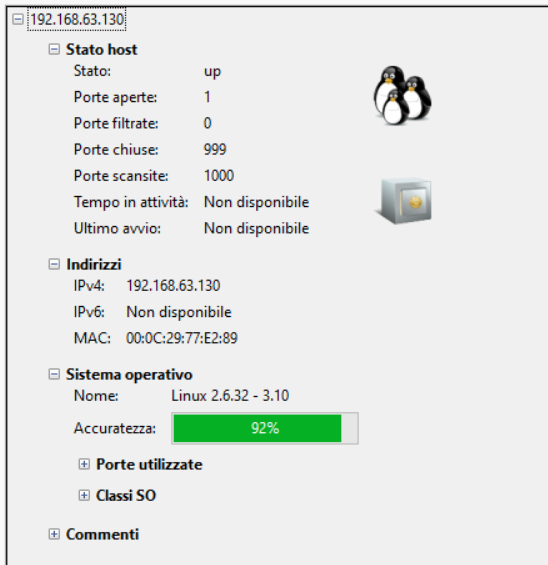
\includegraphics[scale=0.85]{figures/primo_nmap.png}
	\caption{Risultato di Nmap}
	\label{primo_nmap}
\end{figure}

Come si può evincere dall'immagine, viene riconosciuta una versione di Linux non corrispondente a quella attualmente in uso. Quest'operazione è possibile effettuarla eseguendo il seguente comando sul terminale:
\begin{lstlisting}[caption={Comando per mostrare la versione attualmente in uso}]
	hostnamectl
\end{lstlisting}
Visionando ulteriormente il risultato, si può notare come siano state rilevate sia porte aperte che porte chiuse. Questo consente una maggiore precisione nel fingerprinting perché i test vengono effettuati su entrambe le condizioni delle porte, individuate precedentemente tramite port scanning; è quindi logico che evitare questa situazione consente di influenzare parecchio il risultato del fingerprinting.
\\
Per poter evitare la situazione appena descritta, occorre quindi che l'host rifiuti tutti i pacchetti ricevuti che non abbiano come porta destinazione 80 (Well-Known port corrispondente al protocollo applicativo HTTP).
\\
Si procede quindi inserendo una semplice regola nella tabella input delle nftables:

\begin{lstlisting}[caption={Regola per il blocco di tutti i pacchetti ricevuti non diretti alla porta 80}]
	tcp dport != 80 drop
\end{lstlisting}

Con l'utilizzo di questa regola, tutte le porte che prima risultavano \textit{chiuse} ora risultano \textit{filtrate}; la mancanza di test per pacchetti inviati alle porte filtrate influenza pesantemente il risultato del fingerprinting.

\begin{figure}[H]
	\centering
	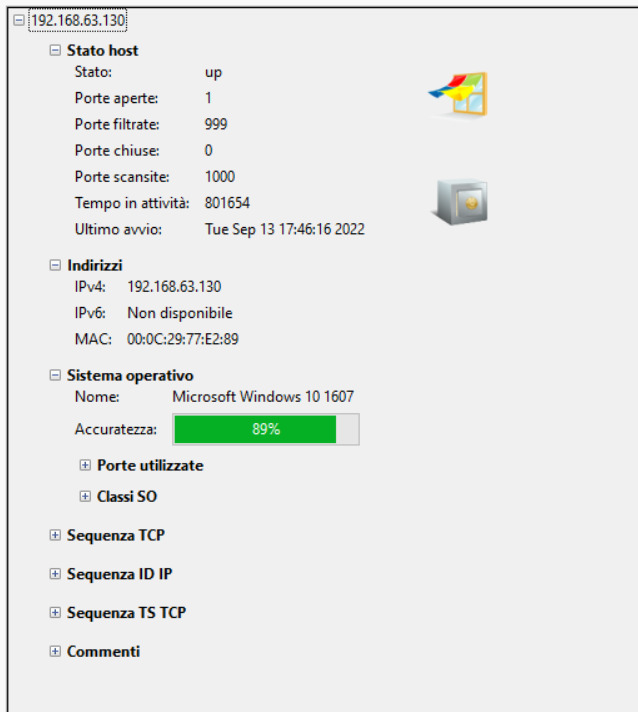
\includegraphics[scale=0.85]{figures/windows_nmap.png}
	\caption{Risultato di Nmap dopo il filtraggio dei pacchetti non diretti alla porta 80}
	\label{windows_nmap}
\end{figure}

Si tratta di un fingerprinting che Nmap definisce "aggressivo", dovuto al fatto che parecchi test non è stato possibile eseguirli; anche per questa ragione la percentuale di sicurezza di Nmap è 89\%, un valore elevato ma che testimonia l'assenza di una certezza assoluta.
Si può quindi affermare che la mancanza di porte chiuse in favore di quelle filtrate sia una strategia utile a contrastare il fingerprinting attivo, diminuendo di fatto i controlli che possono essere effettuati sui pacchetti.

\section{Offuscamento da fingerprinting passivo}
Le tecniche seguite per ingannare i tool di fingerprinting passivo non presentano numerose differenze rispetto a quelle della sezione 4.3; vi è però da considerare il fatto che i pacchetti analizzati non sono ricevuti in risposta a determinati probe.
Questo rende alcune regole impostate precedentemente non più funzionanti, come ad esempio la \ref{codice_icmp}; in questo caso, infatti, l'host non riceve alcun pacchetto echo request con campo code impostato a 9.
\\
Segue l'analisi del database di p0f, presente nel file al percorso /etc/p0f/p0f.fp, con i risultati dei test e le possibilità per un eventuale offuscamento. L'elenco dei campi è specificato nella documentazione offerta da p0f \footnote{Marek, \textit{p0f v3: passive fingerprinter}.}, e si basa sui pacchetti SYN dell'handshake TCP. 
\begin{lstlisting}[caption={Fingerptinting TCP con p0f}]
sig = ver:ittl:olen:mss:wsize,scale:olayout:quirks:pclass

label = s:unix:Linux:3.11 and newer
sig   = *:64:0:*:mss*20,10:mss,sok,ts,nop,ws:df,id+:0
sig   = *:64:0:*:mss*20,7:mss,sok,ts,nop,ws:df,id+:0

label = s:win:Windows:XP
sig   = *:128:0:*:16384,0:mss,nop,nop,sok:df,id+:0
sig   = *:128:0:*:65535,0:mss,nop,nop,sok:df,id+:0
sig   = *:128:0:*:65535,0:mss,nop,ws,nop,nop,sok:df,id+:0
sig   = *:128:0:*:65535,1:mss,nop,ws,nop,nop,sok:df,id+:0
sig   = *:128:0:*:65535,2:mss,nop,ws,nop,nop,sok:df,id+:0
\end{lstlisting}

Il primo valore di cui si può notare la differenza si trova in corrispondenza del campo \textit{ittl}, corrispondente al Time To Live iniziale.
Si tratta di un campo che è possibile modificare per ottenere un offuscamento modificando il file sysctl.conf come descritto al listing \ref{listing_ttl}.
Per quanto riguarda il campo wsize (riferito al Window Size), anche qui vi sono delle diversità, così come per il valore del Window Scaling; entrambi questi valori sono modificabili tramite le regole descritte al listing \ref{listingsize} e \ref{listingscaling}.
Infine, si può riscontrare una differenza nelle opzioni TCP (campo olayout); queste, infatti, non vengono valutate solamente sul loro utilizzo ma anche nell'ordine in cui queste vengono presentate. È evidente che l'ordinamento utilizzato dai due sistemi operativi sia differente, ma purtroppo non è stato trovato alcun modo per modificare quest'ultime.\\
Nonostante ciò, p0f non possiede un meccanismo di punteggio come Nmap, e non mostra il sistema operativo più simile a quello effettivamente testato. Questa caratteristica consente quindi di ottenere un offuscamento anche apportando modifiche minime al fine di determinare un nuovo comportamento del sistema operativo che non sia riconducibile a nessuna riga del database.

P0f analizza inoltre anche il fingerprinting del secondo pacchetto di un handshake TCP (SYN+ACK).

\begin{lstlisting}[caption={Database fingerprinting per pacchetti SYN+ACK dell'handshake TCP}]	
	sig = ver:ittl:olen:mss:wsize,scale:olayout:quirks:pclass

	label = s:unix:Linux:3.x
	sig   = *:64:0:*:mss*10,0:mss:df:0
	sig   = *:64:0:*:mss*10,0:mss,sok,ts:df:0
	sig   = *:64:0:*:mss*10,0:mss,nop,nop,ts:df:0
	sig   = *:64:0:*:mss*10,0:mss,nop,nop,sok:df:0
	sig   = *:64:0:*:mss*10,*:mss,nop,ws:df:0
	sig   = *:64:0:*:mss*10,*:mss,sok,ts,nop,ws:df:0
	sig   = *:64:0:*:mss*10,*:mss,nop,nop,ts,nop,ws:df:0
	sig   = *:64:0:*:mss*10,*:mss,nop,nop,sok,nop,ws:df:0
	
	label = s:win:Windows:7 or 8
	sig   = *:128:0:*:8192,0:mss:df,id+:0
	sig   = *:128:0:*:8192,0:mss,sok,ts:df,id+:0
	sig   = *:128:0:*:8192,8:mss,nop,ws:df,id+:0
	sig   = *:128:0:*:8192,0:mss,nop,nop,ts:df,id+:0
	sig   = *:128:0:*:8192,0:mss,nop,nop,sok:df,id+:0
	sig   = *:128:0:*:8192,8:mss,nop,ws,sok,ts:df,id+:0
	sig   = *:128:0:*:8192,8:mss,nop,ws,nop,nop,ts:df,id+:0
	sig   = *:128:0:*:8192,8:mss,nop,ws,nop,nop,sok:df,id+:0
\end{lstlisting}

Osservando il database si può immediatamente notare come le differenze siano molto simili, in parte uguali, a quelle descritte nel listing precedente.
Le strategie per ottenere l'offuscamento rimangono dunque le medesime.








\chapter{Analisi handshake TLS}
I livelli analizzati in precedenza consentono una corretta comunicazione, ignorando però aspetti importanti quali confidenzialità, integrità ed autenticità; vi è quindi il bisogno di estendere lo stack introducendo un nuovo layer, facoltativo, in grado di garantire queste caratteristiche.
Questo livello viene posizionato tra quello di trasporto e quello applicativo. 

\begin{table}[h]
	\centering
	\begin{tabular}{| l | c |}
		\hline
		Livello 7 & Applicativo
		\\
		\hline
		\rowcolor{yellow!10}Livello 5 & Sicurezza
		\\
		\hline
		Livello 4 & Trasporto
		\\
		\hline
		Livello 3 & Rete
		\\
		\hline
		Livello 2 & Fisico
		\\
		\hline
		
	\end{tabular}
	\caption{Livelli dello stack con layer di sicurezza}
	\label{tab:stackTLS}
\end{table}

Per garantire la confidenzialità dei dati in rete, ovvero la loro segretezza, si fa uso della crittografia ovvero una procedura che modifica i pacchetti in modo da renderli incomprensibili ad attori esterni alla comunicazione.
Questa avviene solitamente in forma simmetrica, ovvero la chiave per cifrare i dati è la medesima utilizzata per decifrarli.

\section{Handshake TLS}
La presenza di una chiave comune ad entrambi i partecipanti della comunicazione pone il problema di come questi ne vengano a conoscenza, non potendosi effettuare lo scambio di chiavi sul medesimo canale delle comunicazioni ordinarie in quanto insicuro.
Oltre alla confidenzialità della chiave, si ha inoltre il problema dovuto all'autenticità della stessa; un eventuale attaccante potrebbe infatti intromettersi nella comunicazione prendendo il posto di uno dei due host, all'insaputa dell'altro (attacco Man In The Middle, MITM).

TLS è un protocollo che prevede uno scambio di messaggi precedente all'invio dei dati veri e propri (handshake) che permette una successiva comunicazione sicura. Si precisa che i pacchetti inviati a questo scopo non sono cifrati, non essendoci ancora una chiave di cifratura in possesso degli host. Solo al termine di questa procedura si saranno scambiate correttamente le chiavi.

Il primo messaggio è inviato dal client al server e prende il nome di \textit{client hello}. In questo messaggio vengono inviate informazioni quali cifrari supportati (in ordine di preferenza), versione TLS in uso, ed estensioni che specificano altri aspetti come ad esempio il supporto alle curve ellittiche o a determinati algoritmi di hashing per il controllo dell'autenticità.

Il server risponde indicando il cifrario da utilizzare, le estensioni da lui supportate, il suo certificato (per garantire l'autenticità della risposta) oltre ad iniziare lo scambio di chiavi, effettuato sfruttando meccanismi matematici in grado di garantire la confidenzialità di quest'ultima anche in caso di MITM passivo.
A questo punto il client termina lo scambio di chiavi.

\section{Browser fingerprinting}
L'analisi delle differenze nel contenuto dei pacchetti client hello inviati da differenti client permette di notare differenze peculiari di quest'ultimi, consentendone la sua individuazione; in questo documento saranno analizzati i browser più popolari.
\\

I browser analizzati sono stati i seguenti:
\begin{itemize}
	\item Chrome versione 105.0.5195.127
	\item Mozilla Firefox versione 105.0
	\item Microsoft Edge versione 105.0.1343.42
	\item Opera versione 91.0.4516.20
\end{itemize}
Non è stato preso in considerazione Safari, in quanto non vi è una versione aggiornata per Windows.
\\

Nel processo di analisi sono stati ispezionati i cifrari utilizzati, l'utilizzo del GREASE, gli algoritmi di hashing supportati e altre estensioni come ad esempio il supporto alle curve ellittiche.

Esaminando i cifrari supportati, si può notare la loro differenza in numero:
\\
\begin{table}[h]
	\centering
	\begin{tabular}{| l | c |}
		\hline
		\rowcolor{yellow!10}Chrome & 16
		\\
		\hline
		\rowcolor{orange!10}Firefox & 17
		\\
		\hline
		\rowcolor{blue!10}Edge & 17
		\\
		\hline
		\rowcolor{red!10}Opera & 16
		\\
		\hline
		
	\end{tabular}
	\caption{Cifrari supportati dai vari browser}
	\label{tab:cifrari}
\end{table}
Questo rende Edge e Firefox differenti rispetto agli altri due, in quanto supportano un numero di cifrari diverso. Firefox, però, presenta anche altre differenze rispetto agli altri come per esempio il supporto ad un maggior numero di algoritmi di hashing e la non presenza del GREASE nei cifrari. 
Per quanto riguarda il primo valore, Firefox è l'unico a presentare un numero diverso rispetto agli altri:

\begin{table}[H]
	\centering
	\begin{tabular}{| l | c |}
		\hline
		\rowcolor{yellow!10}Chrome & 8
		\\
		\hline
		\rowcolor{orange!10}Firefox & 11
		\\
		\hline
		\rowcolor{blue!10}Edge & 8
		\\
		\hline
		\rowcolor{red!10}Opera & 8
		\\
		\hline
		
	\end{tabular}
	\caption{Algoritmi di hashing supportati}
	\label{tab:hash}
\end{table}

Il GREASE,  acroninimo di Generate Random Extensions And Sustain Extensibility, è un valore che corrisponde ad un cifrario inesistente nella realtà e che quindi il ricevente deve ignorare; il protocollo prevede infatti che se il server non supporta un cifrario nella lista questo vada ignorando, valutando quello successivo. Si tratta perciò di un test utile per prevenire bug.
È quindi logico che il GREASE venga posizionato in cima alla lista dei cifrari, in modo che sia sempre valutata dal server.
\\
Anche in questo caso, Firefox è l'unico browser a comportarsi differentemente rispetto agli altri:
\\
\begin{table}[h]
	\centering
	\begin{tabular}{| l | c |}
		\hline
		\rowcolor{yellow!10}Chrome & Sì
		\\
		\hline
		\rowcolor{orange!10}Firefox & No
		\\
		\hline
		\rowcolor{blue!10}Edge &Sì
		\\
		\hline
		\rowcolor{red!10}Opera & Sì
		\\
		\hline
		
	\end{tabular}
	\caption{Presenza del GREASE nella lista dei cifrari supportati}
	\label{tab:grease}
\end{table}

Analizzando nel dettaglio il client hello inviato da Edge, si può notare una caratteristica piuttosto peculiare. Vi è infatti un cifrario, per l'esattezza il \textbf{AES 256 GCM SHA384}, che viene ripetuto due volte all'interno della lista dei cifrari. Questo è ovviamente inutile, in quanto se il server rifiuta quest'ultimo poi procederebbe a valutarlo nuovamente, producendo quindi un nuovo rifiuto. Si tratta dell'unico browser dei quattro che ha questo comportamento, che lo rende molto vulnerabile al fingerprinting.
Di seguito lo screenshot di Wireshark che mostra questa caratteristica.

\begin{figure}[h]
	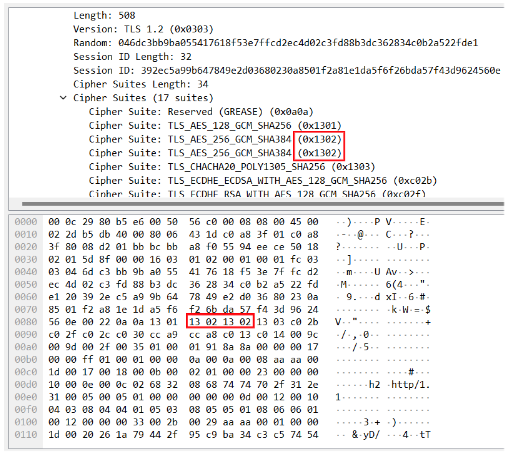
\includegraphics[width=\textwidth]{figures/cifrario_ripetuto.png}
	\caption{Pacchetto client hello inviato tramite Microsoft Edge}
	\label{cifrario_ripetuto}
\end{figure}

Questo causa una differenza di comportamento tra Chrome e Firefox, agevolando il loro riconoscimento. Eliminare il cifrario ripetuto porterebbe Edge ad una situazione uguale a quella di Chrome e Opera, rendendoli quindi indistinguibili.



 









\chapter{Conclusioni}

% PAGINA VUOTA
%\clearpage\null\thispagestyle{empty}\clearpage
%\appendix
%\appendixpage
%\addappheadtotoc

\clearpage\null\thispagestyle{empty}\clearpage


\listoffigures


\begin{flushleft}
\bibliographystyle{plain}
\bibliography{sections/references} 
\end{flushleft}

\end{document}
